\documentclass[../ap_2022.tex]{subfiles}

\graphicspath{{./image/}}

\begin{document}

\setcounter{chapter}{2}
\chapter{統計力学: 合金}
\section{}
\(N_A\)A原子にとって最近接の原子を1個見たときにそれが原子Bになる確率は\(N_B/N\)で、
最近接は\(z\)だけある。なので
\begin{equation}\begin{aligned}[b]
    N_{AB}&=zNA\frac{N_B}{N}=x(1-x)zN\\
    E &= x(1-x)zNV
\end{aligned}\end{equation}

\section{}
ボルツマンエントロピーを考える。\(N\)個ある格子点の中から原子Aを\(N_A\)個配置する方法は\(~_NC_{N_A}\)であるのでエントロピーは
\begin{equation}\begin{aligned}[b]
    S = k_B \ln\frac{N!}{N_A!N_B!} \simeq k_B\qty[N\ln N-N_A\ln N_A -N_B\ln N_B]
    =-Nk_B\Bigl(x\ln x+(1-x)\ln(1-x)\Bigr)
\end{aligned}\end{equation}

\section{}
ヘルムホルツの自由エネルギーは
\begin{equation}\begin{aligned}[b]
    F = E-TS = N\Bigl(
        x(1-x)zV+k_BT\qty[x\ln x+(1-x)\ln(1-x)]
    \Bigr)
\end{aligned}\end{equation}

\section{}
\(f(x)\)の極地は
\begin{equation}\begin{aligned}[b]
    0 &= f'(x) = (1-2x)zV +k_BT\ln\frac{x}{1-x}\\
    \frac{zV}{k_BT}(2x-1) &= \ln\frac{x}{1-x}
\end{aligned}\end{equation}
より
\begin{equation}\begin{aligned}[b]
    g(x) = \ln\frac{x}{1-x}
\end{aligned}\end{equation}

\section{}
\(g(x)\)の\(x=1/2\)における傾きは
\begin{equation}\begin{aligned}[b]
    g'(1/2) &= \frac{1}{1/2}+\frac{1}{1-1/2} = 4
\end{aligned}\end{equation}
これが式(2)の左辺の傾きと等しいので
\begin{equation}\begin{aligned}[b]
    \frac{2zV}{k_BT_{c0}}&=4\\
    T_{c0} &= \frac{zV}{2k_B}
\end{aligned}\end{equation}


\section{}
以下の図1の通りである。
\begin{figure}[h]
    \centering
    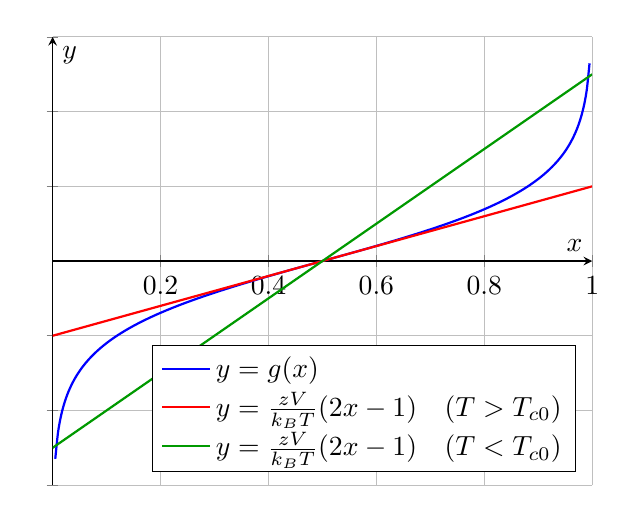
\begin{tikzpicture}
                \begin{axis}[
            axis lines=middle,          % 座標軸を中央に配置
            xlabel=$x$,                 % x軸ラベル
            ylabel=$y$,                 % y軸ラベル
            xmin=0, xmax=1,             % x軸の範囲
            ymin=-6, ymax=6,            % y軸の範囲
            grid=major,                 % 目盛り線を表示
            legend pos=south east,% 凡例をグラフの右上外側に配置
            legend cell align={left},   % 凡例のテキストを左揃えに
            samples=200,                % プロットのサンプル数
            smooth,                     % 曲線を滑らかに描画
            yticklabels={},             % y軸の値を非表示
        ]

        % y = log(x/(1-x)) のグラフ (青色)
        \addplot[
            domain=0.005:0.995, % 定義域 (0,1) を考慮し、端点を避ける
            color=blue,
            thick,
        ] {ln(x/(1-x))};
        \addlegendentry{$y =g(x)$}

        % y = a(2x-1) のグラフ

        % a = 2 の場合 (赤色)
        \addplot[
            domain=0:1,
            color=red,
            thick,
        ] {2*(2*x - 1)};
        \addlegendentry{$y = \frac{zV}{k_BT}(2x-1)\quad (T>T_{c0})$}

        % a = 5 の場合 (緑色)
        \addplot[
            domain=0:1,
            color=green!60!black,
            thick,
        ] {5*(2*x - 1)};
        \addlegendentry{$y = \frac{zV}{k_BT}(2x-1)\quad (T<T_{c0})$}
        \end{axis}
    \end{tikzpicture}
    \caption{設問[6]の回答}
\end{figure}

\section{}
\begin{equation}\begin{aligned}[b]
    0 &= f''(x)=-2zV + \frac{k_BT}{x(1-x)}\\
    \frac{k_BT}{2zV} &=x(1-x)\\
    &=\frac{1}{4}-\delta_1^2 \\\
    \delta_1 &= \pm\sqrt{\frac{1}{4}-\frac{k_BT}{2zV}}
\end{aligned}\end{equation}

\section{}
以下の図2の通りである。
\begin{figure}[h]
    \centering
    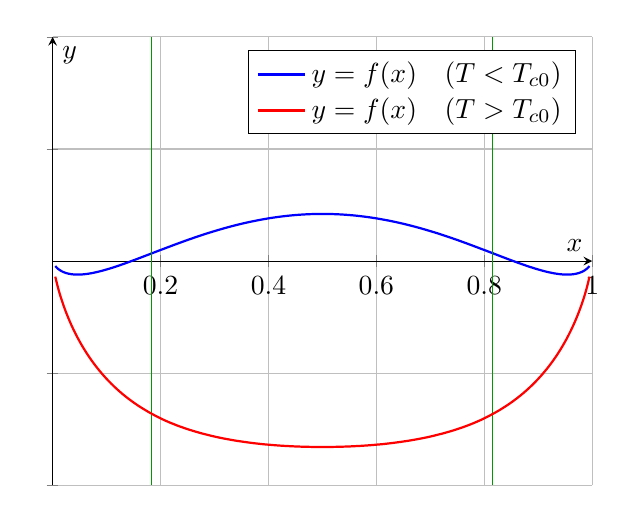
\begin{tikzpicture}
                \begin{axis}[
            axis lines=middle,          % 座標軸を中央に配置
            xlabel=$x$,                 % x軸ラベル
            ylabel=$y$,                 % y軸ラベル
            xmin=0, xmax=1,             % x軸の範囲
            ymin=-0.2, ymax=0.2,            % y軸の範囲
            grid=major,                 % 目盛り線を表示
            legend pos=north east,% 凡例をグラフの右上外側に配置
            legend cell align={left},   % 凡例のテキストを左揃えに
            samples=200,                % プロットのサンプル数
            smooth,                     % 曲線を滑らかに描画
            yticklabels={},             % y軸の値を非表示
        ]

        % y =f(x) 低温のグラフ (青色)
        \addplot[
            domain=0.005:0.995, % 定義域 (0,1) を考慮し、端点を避ける
            color=blue,
            thick,
        ] {x*(1-x) + 0.3*(x*ln(x) + (1-x)*ln(1-x))};
        \addlegendentry{$y =f(x)\quad (T<T_{c0})$}

        \draw [solid, color=green!60!black] (axis cs:0.184, \pgfkeysvalueof{/pgfplots/ymin}) -- (axis cs:0.184, \pgfkeysvalueof{/pgfplots/ymax});
        \draw [solid, color=green!60!black] (axis cs:0.816, \pgfkeysvalueof{/pgfplots/ymin}) -- (axis cs:0.816, \pgfkeysvalueof{/pgfplots/ymax});

         \addplot[
            domain=0.005:0.995, % 定義域 (0,1) を考慮し、端点を避ける
            color=red,
            thick,
        ] {x*(1-x) + 0.6*(x*ln(x) + (1-x)*ln(1-x))};
        \addlegendentry{$y =f(x)\quad (T>T_{c0})$}

        \end{axis}
    \end{tikzpicture}
    \caption{設問[8]の回答\url{https://www.desmos.com/calculator/opyewmm4vp?lang=ja}}
\end{figure}

\section{}
\(\frac{1}{2}\pm\delta_0(T)\)の方が
\(\frac{1}{2}\pm\delta_1(T)\)よりも早く1に近づくような図を描く。

\section{}
\begin{equation}\begin{aligned}[b]
    x_0 &= sx_1+(1-s)x_2\\
    s &= \frac{x_0-x_2}{x_1-x_2}
\end{aligned}\end{equation}

\section{}
\begin{equation}\begin{aligned}[b]
    f^* = sf(x_1)+(1-x)f(x_2) = \frac{x_0-x_2}{x_1-x_2}f(x_1)\frac{x_1-x_0}{x_1-x_2}f(x_2)
\end{aligned}\end{equation}

\section{}
\begin{equation}\begin{aligned}[b]
    f^* &= \frac{x_0-x_0-\delta}{-2\delta}f(x_0-\delta)+\frac{x_0-\delta-x_0}{-2\delta}f(x_0+\delta)\\
    &=\frac{f(x_0-\delta)+f(x+\delta)}{2} \\
    &\simeq f(x_0)+\frac{1}{2}f''(x_0)\delta ^2
\end{aligned}\end{equation}
これが式(3)を満たすので、
\begin{equation}\begin{aligned}[b]
    f''(x_0)>0
\end{aligned}\end{equation}
とわかる。

\section{}
設問[9]の図で\(x=x_0\)の線を引くと、
\(\frac{1}{2}\pm\delta_0(T)\)と
\(\frac{1}{2}\pm\delta_1(T)\)によって
\(x=x_0\)の線が分割されて、
左の低温から順に領域III, 領域II, 領域I になる

\section*{感想}
結晶作ってる人は合金の相図が頭に入ってるはずなので、
そうなると問題文の把握も回答もやりやすい問題なのでしょうね。
私は実験やったことないので、変なところで勘違いしてたりしてました。

\end{document}
